\color{cyan} %color de texto con 70-80 % o más de avance
\section{Sensado remoto, plataformas (Bloque 1)}
\subsection{Fotointerpretación}
En el marco de la teledetección, la fotointerpretación consiste en el análisis de imágenes, generalmente aéreas sobre un terreno, para extraer información, identificar objetos, clasificar, etc. Se parte de una captura de fotogramas, mediante alguna plataforma que puede ser una aeronave tripulada o no, o un satélite. Durante un tiempo la fotointerptretación era llevada a cabo de manera manual, valiéndose el fotointerpretador de una imagen impresa y herramientas como estereoscopio, reglas, marcadores. Con la mayor accesibilidad y disponibilidad de herramientas digitales, se vuelve más atractivo el uso de métodos que automaticen la tarea.

En el caso de las imágenes aéreas es muy probable que sean necesarias varias imágenes para cubrir la zona de interés. Si se pretende construir un ortomosaico con esas imágenes, es necesario garantizar al momento de realizar las capturas un mínimo nivel de solapamiento entre capturas consecutivas (60\%) y entre aquellas que pertenecen a líneas de vuelo adyacentes (25\%). Los satélites son básicamente cámaras que orbitan alrededor del planeta que capturan imágenes de manera regular, continua, las cuales se  almacenan temporalmente en el satélite y son descargadas a estaciones de enlace para luego ser comercializadas. De modo que a requerimiento, las imágenes suelen estar disponibles. diferente es el caso de las imágenes aéreas, para las cuales se define un vuelo específico- Eso conlleva otros tiempos, ya que implica programar y preparar el vuelo, eventualmente trasladar la aeronave si es tripulada desde el aeródromo del cual despega y al cual regresa para aterrizar, y la duración misma del procedimiento de captura. Entre las variables que intervienen en la duración del vuelo en la fase de captura de imágenes se puede mencionar la de la extensión del área de interés, la velocidad de desplazamiento, la altura de vuelo. Esto también tendrá incidencia en la resolución espacial de las imágenes y en el espacio de almacenamiento requerido. Finalmente en el costo total del procedimiento, en el caso de aeronaves tripuladas incidirá el tiempo que lleve desde la puesta en marcha del motor hasta su apagado, ya que todo eso se contempla como hora de vuelo.
Los sensores, esto es, las cámaras que son llevadas como carga útil por las diferentes plataformas, están definidos por sus características. La distancia focal es un atributo de cada cámara. El factor de escala está dado por la altura de vuelo sobre el terreno, que puede variar incluso durante el vuelo, y por la distancia focal de la cámara, que es fija. 
\begin{figure}
    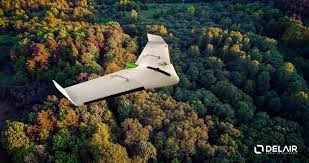
\includegraphics[width=\textwidth]{Imagenes/dron.jpg}
     \hfill
     \caption{Acá puede ir o no una imagen ilustrativa; revisar que esté referenciada correctamente}
    \label{dron}
\end{figure}

\subsection{Plataformas para el sensado remoto}
En este apartado se analizarán las principales características de las opciones de plataformas para el sensado remoto. El análisis se limitará a la opción de uso de sensores de espectro visible.
Los sensores remotos que serán tratados en el presente trabajo son del tipo pasivo, es decir, están compuestos por detectores que registran las ondas de luz solar reflejadas en el terreno. Particularmente nos interesan los que cubren el espectro visible. Básicamente constituyen una cámara fotográfica, que se compone de un arreglo de lentes y espejos que refractan y reflejan la luz, proyectándola sobre un sensor fotosensible, generalmente es un rectángulo conformado como un arreglo de detectores, cada uno de ellos representa a un pixel de la imagen. Según las características de estos sensores y la configuración de lentes, la distancia al objetivo, la resolución espacial queda determinada. 
\subsubsection{Imaginería satelital}
Se entiende por satélite artificial a todo dispositivo fabricado por el humano que es puesto en órbita alrededor del planeta Tierra con diversos propósitos que abarcan desde el establecimiento de comunicaciones hasta la observación terrestre por medio del sensado remoto. Éste último es el que reviste interés para el presente trabajo. Los satélites para sensado remoto van generalmente equipados con sensores multiespectrales, con múltiples bandas. La operación de los satélites es de manera continua desde que son puestos en órbita hasta el fin de su vida útil, varios años después. El lanzamiento y puesta en órbita requiere de infraestructura adecuada a tal fin, de las cuales hay muy pocas en el mundo, concentradas en no más de una decena de países. Los datos recopilados por los satélites son transmitidos a estaciones terrenas ubicadas en distintos puntos del planeta, y el acceso a las imágenes de alta resolución suele ser restringido a una contraprestación monetaria. No obstante suele haber acceso gratuito a imágenes con menor resolución. Las imágenes satelitales se definen por sus características de resolución, que son cuatro: resolución espacial, espectral, temporal y radiométrica.

Según la base de datos de la Unión de Científicos Conscientes \cite{noauthor_satellite_nodate}, actualizada el primero de mayo de 2.022, existen alrededor de 5.500 satélites orbitando la Tierra, de los cuales 1.156 (es decir un 21\%)tienen por finalidad la observación terrestre. Son utilizados varios tipos de sensores considerando el rango de frecuencias o la longitud de onda para cuya adquisición han sido diseñados. Se destacan los de luz visible, infrarrojo cercano (near infrared - NIR), infrarrojo térmico (thermal infrared - TIR), pancromático e infrarrojo de onda corta (shortwave infrared - SWIR). También existe un considerable despliegue de radares de apertura sintética (synthetic aperture radar - SAR) en diferentes bandas. De los satélites de observación terrestre, aproximadamente un 40\% son con sensores ópticos, es decir, capturan imágenes en el espectro visible.
Hay muchas y muy diversas fuentes de imágenes satelitales, tanto en forma gratuita como pagas. Entre las opciones pagas, imágenes multiespectracles con una resolución espacial de 50 cm se consiguen por montos entre 10 dólares por km\textsuperscript{2} hasta 29 dólares por km\textsuperscript{2} según sean actualizadas o de archivo (más de 90 días)\cite{noauthor_satellite_2020}. Debe tenerse en cuenta el tamaño mínimo del área a ser adquirida, en caso de las imágenes de archivo son 25 km\textsuperscript{2} (2500 ha) y las actualizadas son de 100 km\textsuperscript{2} (10000 ha).
\begin{table}[H]
    \centering
    \caption{Características de sensores satelitales. Fuente \cite{noauthor_3_nodate}}
    \begin{tabular}{|c|p{20mm}|p{15mm}|p{15mm}|p{25mm}|p{20mm}|p{20mm}|p{20mm}|}
        \hline
        \textbf{Sensor} & \textbf{Tamaño de imagen} & \multicolumn{4}{c}{\textbf{Resolución}} & \textbf{Aplicación principal} \\
        %\hline
        & & \textbf{Espacial} & \textbf{Temporal} & \textbf{Radiométrica} & \textbf{Espectral}  &\\
        \hline \hline
        Meteosat & Toda la esfera & 	2500 m 	& 0.5 h 	& 256 ND 	& 1Vis 1IR 1 IT & Meteorología\\
        \hline
        NOAA AVHRR & 2700 x 2700 km	& 1100 m 	 	& 12 h 	& 1024 ND 	& 2Vis 1IR 1IT & Observación atmosférica\\
        \hline
        Landsat TM 	& 185 x 185 km & 30 m 	 	& 16 d 	& 256 ND 	& 3Vis 3IR 1IT & Observación terrestre\\
        \hline
        SPOT HRV & 60 x 60 km	& 20 m 	 	& 20 d	& 256 ND 	& 2Vis 1IR & Observación terrestre\\
        \hline
        SPOT Vegetation & 2200 x 200 km	& 1150 m 	 	& 1 d	& 1024 ND 	& 2Vis 2IR & Monitoreo agrícola\\
        \hline
        MODIS & 2330 x 2330 km	& 250 - 100 m 	 km 	& 1 d	& 1024 ND 	& 36 bandas & Observación terrestre\\
        \hline
        IKONOS & 100 x 100 km	& 4 m 	 	& 3 d 	& 2048 ND 	& 3Vis 1IR & Observación terrestre\\
        \hline
        Albedo & 35 x 7 km & 0,4 m  & 1 d & S/D & 3Vis 1IR & Observación terrestre\\
        \hline
         Worldview & 13 x 13 km &   & 1 d & 2048 & 29 bandas & Observación terrestre\\
        \hline
         Sentinel & 13 x 13 km &  10 m & 1 d & S/D & 13 bandas & Observación terrestre\\
        \hline
    \end{tabular}

\label{Satelites}
\end{table}
\subsubsection{Aeronaves convencionales tripuladas}
Aquí se agrupan las aeronaves de determinado porte, cuya operación debe hacerse con tripulación, requiriendo que sea personal capacitado y con licencia para operarlos. En esta categoría se incluyen los aviones de ala fija, como los de ala rotatoria (helicópteros) así como aerostatos. Su operación requiere de una planificación de vuelo que debe ser reportada al área de espacio de vuelo controlado, además de necesitar una base de despegue y aterrizaje. El marco regulatorio de estas operaciones son las Regulaciones Argentinas de la Aviación Civil (RAAC), Parte 91 \cite{noauthor_infoleg_nodate-1}.
\paragraph{Cámaras fotográficas}
Algunos tipos de cámaras utilizadas a bordo de aeronaves tripuladas para realizar relevamientos fotogramétricos:
Vexcel UltraCam Eagle

%Se podría añadir como figura un mapa con las regiones de información de vuelo (FIR), con las zonas de control, aeródromos habilitados, por ejemplo, etc.
\subsubsection{Aeronaves no tripuladas}
Generalmente conocidos como VANT, los vehículos aéreos no tripulados (VANT) son cada vez más asequibles por el público general. Disponibles en amplia variedad de modelos, constituyen una formidable herramienta para llevar a cabo tareas de relevamiento aéreo. El abanico de posibilidades se ve ampliado por la prescindencia de una pista de despegue o aterrizaje de dimensiones grandes. El marco legal regulatorio para la actividad con VANT es la resolución ANAC 885 \cite{noauthor_infoleg_nodate}.
Existe una amplia variedad de tipos de VANT, que pueden ser de múltiples rotores o de ala fija. El propósito del presente trabajo no es exhaustivo en este aspecto, pero a los efectos de describir las características principales, se lo hará con algunos de ellos.
\paragraph{Multirrotor}
Los VANT tipo multirrotor poseen cuatro o más hélices para proporcionar al vehículo la sustentación y la propulsión en tres ejes de desplazamiento. Esta característica es la que le confiere mayor maniobrabilidad, especialmente en espacios reducidos. La energía para propulsarse es eléctrica, proveniente de baterías. Son los más difundidos comercialmente.
\subparagraph{DJI Mini 2}
Un dron comercial asequible es el Mini 2 del fabricante DJI \cite{noauthor_dji_nodate-1}. Está equipado con una cámara con sensor 1/2.3” CMOS, de 12 millones de píxeles efectivos. La lente de la cámara posee un ángulo de visión de 83º y un formato equivalente a 35 mm de longitud focal de 24 mm, una apertura de f/2.8 y un rango focal de 1 m hasta infinito. En cuanto a las velocidades, el dron tiene tres modos de funcionamiento, modo Sport, modo Normal y modo Cine. En Sport se desplaza hasta 16 m/s, en modo normal 10 m/s y en modo cine 6 m/s.
\subparagraph{DJI Mavic 3M}
Este es un dron profesional \cite{noauthor_dji_nodate}. Cuenta con una cámara RGB de 4/3 CMOS, con 20 millones de píxeles efectivos. La lente es de un campo de visión de 84º, con una longitud focal equivalente de 24 mm. La apertura es de f/2.8 a f/11, y foco de 1 m al infinito. En modo normal puede desplazarse hasta 15 m/s
\paragraph{Ala fija}
Este tipo de VANT poseen un ala fija que le brinda sustentación, por lo que pueden incluso planear aunque falle la planta motriz de la aeronave. Sus características de funcionamiento permiten vuelos más extensos, cubriendo mayores áreas. Existen VANT de ala fija alimentados eléctricamente con baterías o con motores de combustión interna. Se los encuentra esencialmente en aplicaciones de agricultura de precisión y en el campo militar. 
\subparagraph{Asesor/9}
Es un VANT de ala fija de casi 2 m de envergadura \cite{noauthor_drone_nodate}. Puede desplazarse a 17 m/s y tiene una autonomía de dos horas de vuelo. Va equipado con una cámara multiespectral MicaSense Altum-PT \cite{noauthor_altum-pt_2023} cuyo sensor es de 12,4 millones de píxeles, que le confieren una resolución de 5,28 cm/pixel volando a 120 m sobre el terreno.

Sensor
12.4 MP sensor pancromático
Cinco bandas espectrales de 3.2 MP
Resolución
Multiespectral (pan-sharpened): 1.24cm/pixel a 60m; 2.49cm/pixel a 120m

RGB12.4 MP (obturador global, alineado con todas las bandas)
Sensor térmicoFLIR LWIR infrarrojo térmico 7.5-13.5um calibrado radiométricamente
RESOLUCIÓN5.28 cm cm / pixel (por banda MS), 33.5 cm / pixel (banda térmica), 2.49 cm / pixel (pancro) a 120 m AGL
VELOCIDAD DE CAPTURAHasta 3 capturas por segundo DNG sin procesar
INTERFACES3 GPIO: señal de disparo, salida de la parte superior del cuadro, salida de 1 PPS, botón host. Puerto USB 2.0 para WiFi, ethernet 10/100/1000, serial, y almacenamiento CFexpress
CAMPO DE VISIÓN50° HFOV x 38° VFOV (MS) / 44° HFOV x 38° VFOV (PAN)
\color{black}
\section{Procesamiento de imágenes (Bloque 2)}

\subsection{Concepto de imagen, espacios de color, entidad matricial)}
El proceso de obtención de imágenes tiene como punto de partida la captura, que consiste esencialmente en un recorte dimensional y temporal que es fijado en una plataforma, antiguamente una solución química, actualmente en forma electrónica. Los sensores de las cámaras fotográficas están dispuestos en un arreglo matricial, de ese modo las imágenes pueden ser representadas por la entidad matemática matriz, cuyos elementos son denominados píxeles. Existen imágenes monocromáticas o multiespectrales. En el primer caso la matriz es bidimensional. En el caso multiespectral será un arreglo multidimensional, el caso más general es el que se compone de tres bandas de color en el espectro visible, rojo, verde y azul, también conocido con el acrónimo RGB del idioma inglés. Bajo esa forma de representación, las imágenes pueden ser procesadas y sometidas a análisis mediante algoritmos computacionales. En general, previo al análisis de imágenes se suele aplicar un preprocesamiento que involucra algún tipo de filtrado, o algún ajuste de parámetros de la imagen, como el contraste. También suele realizarse alguna conversión entre diferentes espacios de color, según los requerimientos.
\subsection{Sombras en dosel selvático}
La presencia de sombras en las imágenes aéreas del dosel selvático puede aportar información sobre la eventual existencia de ejemplares de capa emergente. Asimismo puede ser un signo descriptivo de la estructura de la porción de selva estudiada, evidenciando claros, huecos en la selva que denoten algún tipo de acción extractiva, o la presencia de especies de flora exótica amenazantes.
\subsection{Filtrado homomórfico (Javier)}
\subsubsection{C1-Lógica difusa y procesamiento homomórfico (sombras)}
Según el modelo Stockham \cite{stockham_image_1972} una imagen puede descomponerse en dos partes, una la denominada iluminación y la otra componente es la reflexión. Llevadas al plano de frecuencias, se confirma el hecho de que la componente de iluminación tiene una variación más lenta, es decir, se corresponde con las frecuencias bajas. De modo similar, la componente de reflexión se corresponde con frecuencias altas \cite{oppenheim_nonlinear_1968}. Entendiendo esto, es factible implementar un filtrado en la imagen para realzar las sombras, separando la componente de iluminación de la de reflexión. Esta técnica fue utilizada en la remoción de sombras en imágenes de piezas de manufactura \cite{yang_research_2012} y en la detección automática de sombras en objetos oscuros \cite{etemadnia_automatic_2003}. En el presente trabajo, la aplicación a la detección de especies arbóreas es novedosa. 
\subsection{Procesamiento morfológico (Wagner)}
Una réplica del trabajo de \cite{ferreira_tree_2019}
Partiendo de una imagen en escala de grises, se realizó una secuencia de pasos en los que se implementan diferentes filtros para identificar cada una de las copas, de un modo que finalmente se obtuvo una imagen binarizada con la cual se pudo obtener un conteo de las copas. El primer paso consistió en hacer una clara identificación de los bordes y del área de copas. Luego se aplicó un algoritmo de Rolling Ball \cite{sternberg_biomedical_1983} que produce un suavizado en los niveles de grises dentro de las copas. En una siguiente etapa, distinguiendo copas grandes de pequeñas, se identificaban huecos en las copas grandes, para posteriormente rellenarlos con un valor promedio. Una vez rellenos todos los huecos y uniformadas todas las copas, se procede a segmentarlas, obteniéndose una imagen binarizada, con cada copa de árbol aislada e identificada en su posición.
El tratamiento automático de clasificación de especies arbóreas a partir de imágenes requiere de un conjunto de habilidades informáticas que van desde la manipulación el tratamiento de
las imágenes hasta el entrenamiento de modelos de aprendizaje automático. Para obtener una
aceptable clasificación de copas es necesario realizar procesamiento a la imagen
aprovechando las características de textura y contraste que ésta exhibe. Los algoritmos
matemáticos desarrollados en este trabajo posibilitan una adecuada segmentación de las
copas individuales del dosel y capa emergente de la Selva Atlántica, lo que consecuentemente
habilita en otro nivel la clasificación por especies. Para obtener el segmentado se toma como
punto de partida la imagen aérea en escala de grises, ya que se enfoca en los diferentes
contrastes y texturas existentes entre el área de copas y el espacio entre ellas. Corresponde
hacer una primer etapa de identificación gruesa entre copas y bordes, luego se homogeneiza el
interior de las copas para eliminar huecos. La imagen es tratada matemáticamente como una
matriz donde cada elemento es un píxel, cuyo valor se relaciona con la intensidad
correspondiente al espacio de color HSI. Esta matriz es pasible de manipulación matemática,
de modo que permite aplicársele filtros varios, algoritmos de procesamiento morfológicos, que
permiten resaltar estructuras internas de la imagen, facilitando esto la segmentación de copas.
Se aplica un criterio de distinción de tamaño de copas grandes y chicas, partiendo desde la
resolución espacial de la imagen, definiendo aquellas grandes como las que superan el radio
de tres píxeles. Diferentes algoritmos se aplican de forma secuenciada, procesando sobre los
resultados de cada paso anterior. De modo que intervienen algoritmos de homogeneización
como el filtro RollingBall, el filtrado top-bottom-hat basado en operadores morfológicos de apertura y clausura. En cada etapa se definen parámetros que se ajustan según las condiciones
de la imagen, algunos de los cuales se obtienen por medio de herramientas de estadística
(promedio, percentiles, etc.). Estos son tenidos en cuenta para definir umbrales de decisión. A
los fines de visualizar el comportamiento de los algoritmos y la influencia de estos parámetros,
se condujo una evaluación tipo “gridsearch” en la que se definió un rango para cada parámetro
y se expuso el resultado correspondiente. Esta pasantía se desarrolla en linea con los objetivos
propuestos en el plan de trabajo de la tesis doctoral relacionada con la detección automática
de especies de árboles nativos en la selva atlántica. 
%\color{cyan} %color de texto con 70-80 % o más de avance
\subsection{Invariante de color (paper turco)}
%\color{cyan}
\subsection{C2-Índice invariante de color (sombras)}
Un método que dio resultados interesantes en la detección de sombras es el que implementaba el cálculo del índice invariante de color (IIC). Probando con distintos valores de umbral, se observó que el que producía resultados más satisfactorios era el que correspondía al 85º percentil de la distribución de los valores de IIC.
El punto de partida del método es la adquisición de imágenes aéreas. No hay requerimientos especiales, excepto que se den las condiciones para proyección de sombras. Se tomaron imágenes de un área representativa de la selva nativa en la provincia de Misiones, las cuales fueron capturadas desde un VANT que sobrevoló las áreas de interés. A los efectos de obtener imágenes con presencia de sombras, se estableció un adecuado rango temporal de captura de imágenes, en este caso de 3 a 4 pm. Las imágenes fueron adquiridas en el invierno meridional, en el mes de agosto, cuando la proyección de sombras es mayor debido a la posición relativa del sol. Se utilizó un dron Mini 2, del fabricante DJI, equipado con una cámara de 12 megapíxeles. La altura de vuelo sobre el terreno fue de 50 metros. la resolución espacial de las imágenes son de 3 cm/píxel.
\subsubsection{Introducción IIC}
La conservación de áreas naturales forestales tiene cada vez mayor relevancia a nivel mundial debido a que los bosques nativos tienen un rol probado en la mitigación del cambio climático. En ese sentido se han propuestos numerosas acciones usando diversas herramientas para ayudar a conservar los bosques. Entre dichas herramientas el relevamiento y monitoreo de bosques mediante imágenes aéreas es un campo promisorio. En particular el monitoreo de la Selva Atlántica es un tópico que ha recibido mucha atención en las últimas décadas, desgraciadamente porque se ha convertido en uno de los ecosistemas más amenazados en el mundo. Siendo originalmente de una extensión de 1.290.692,46 km$^2$ durante los últimos siglos, que abarcaba parte de Brasil, Argentina y Paraguay, hoy la Selva Atlántica está reducida a casi 162.000 km$^2$, lo que representa sólo un 12,4 \% de la extensión original \cite{de_lima_erosion_2020}, y se ubica principalmente en la Provincia de Misiones en Argentina. A pesar de de este escenario adverso, la diversidad de especies que habitan en la Selva Atlántica es aún una de las más grandes del mundo \cite{lima_how_2015}. Sin embargo algunas especies de fauna y flora están en un estado de conservación crítico, como por ejemplo algunas especies de árboles cuya copa sobresale del dosel, situándose en lo que se conoce como capa emergente, a treinta metros o más respecto del suelo \cite{noauthor_rainforest_2015}, por lo que sería recomendable conocer la cantidad y geolocalización de este tipo de árboles. También sería de interés determinar la distribución y localización de algunas especies como bambú y lianas, que podrían ser indicadores de niveles de preservación \cite{bedrij_selective_2022}. En este contexto el monitoreo forestal representa un rol crítico en la evaluación de la eficacia de estrategias de restauración, identificando acciones correctivas, comparando resultados entre proyectos y aprendiendo de proyectos pasados para determinar futuros lineamientos en restauración \cite{viani_protocol_2017}
El nivel de preservación de la Selva Atlántica ha sido evaluado con varios métodos. El más difundido es la exploración in situ, restringido a áreas pequeñas, con posibilidad de ser extrapolados los resultados a áreas más grandes con el correspondiente error de estimación. En esta forma tradicional, el monitoreo forestal es una tarea ardua y demandante de tiempo, por lo que al transcurrir el tiempo entre revisitas, las condiciones ambientales podrían haber cambiado de modo considerable. Además el desplazamiento dentro de la selva resulta difícil y puede generar disturbios en la flora y en la fauna locales. Todo esto puede evitarse con el monitoreo forestal por medio de análisis de imágenes aéreas o satelitales. Éstas últimas representan una fuente interesante de datos, principalmente debido al inmenso área que puede cubrir una simple escena (cientos de kilómetros cuadrados) con múltiples bandas espectrales, especialmente más allá del espectro visible. Sin embargo tienen usualmente una relativamente baja resolución espacial y baja disponibilidad. En el mejor de los casos la resolución espacial de estas imágenes está en el orden de 30 cm por pixel \cite{poli_radiometric_2014}, siendo su adquisición onerosa, que puede ser de varios miles de dólares por cada escena \cite{noauthor_geocento_2022}. La obtención de estas imágenes está condicionada a la disponibilidad en el tiempo, ya que en algunos casos la frecuencia de revisita de determinados sitios puede ser de varios días \cite{li_global_2017}.
A pesar de estas desventajas, varios trabajos han relevado especies arbóreas y recolectado datos forestales usando imágenes satelitales con alta resolución espacial y espectral \cite{gomes_detection_nodate,cross_classification_2019,abd_latif_determination_2012,ferreira_tree_2019,radoux_quantitative_2007}. Por otro lado, otros trabajos han monitoreado bosques usando otras herramientas como los vehículos aéreos no tripulados (VANT) \cite{albuquerque_remotely_2020,albuquerque_forest_2021,qin_individual_2022,machida_modeling_2022}, en la detección de flores \cite{campbell_simple_2018} o incorporando sensores LiDAR \cite{terryn_quantifying_2022,brede_non-destructive_2022}. La combinación de imágenes aéreas o satelitales de alta resolución espacial con herramientas computacionales facilita la implementación del mapeo del estado de salud forestal \cite{prost_discrimination_2008} o el conteo automático de árboles \cite{putra_automatic_2023}. Las imágenes aéreas obtenidas con VANT poseen algunas ventajas sobre las satelitales, entre las que se encuentra su relativo bajo costo, su muy alta resolución espacial y su baja altitud de sobrevuelo, lo cual permite evitar interferencias de nubes \cite{alexander_locating_2018,ahmad_aerial_2010,zhang_seeing_2016,ahmad_digital_2013,colomina_unmanned_2014,eisenbeiss_mini_nodate}. No obstante, la combinación de la posibilidad de captura de imágenes de grandes extensiones de selva con una adecuada resolución espacial para luego procesar esas imágenes con métodos y tecnologías que ofrecen resultados aceptables sin excesivas demandas computacionales y requerimientos tecnológicos no es tan sencilla de implementar. La clave para alcanzar esa meta es trabajar con un atributo de la imagen que puede ser extraído con algoritmos eficientes. En este estudio asumimos que puede explorarse la información contenida en regiones sombreadas de imágenes aéreas de regiones forestales mediante algoritmos computacionales de bajo costo.
Las sombras se producen por oclusión por parte de un objeto de forma total o parcial de la luz directa emanada de la fuente \cite{hu_revisiting_2021}. En la bibliografía se considera que las sombras en imágenes de sensado remoto pueden ser originados por tres causas: material natural o urbano (árboles o edificios), características topográficas (colinas o montañas) y nubes \cite{shahtahmassebi_review_2013}. La presencia de sombras en imágenes de sensado remoto es objeto de muchas consideraciones. En algunos casos las sombras pueden ser una fuente de información útil, proveyendo por ejemplo una perspectiva en tres dimensiones de una escena capturada, mientras que en otros casos la presencia de sombras dificulta la recolección de datos detallados. Hay por lo tanto numerosos trabajos sobre el procesamiento de imágenes con sombras \cite{shahtahmassebi_review_2013,mostafa_review_2017,freitas_automatic_2017,chang_c_evaluation_2016}. Algunos trabajos están basados en el modelo de Stockham \cite{stockham_image_1972}, implementando el filtrado homomórfico para la remoción de sombras \cite{yang_shadow_2007} o para la detección de sombras en imágenes aéreas de selvas \cite{bernhardt_deteccion_2017}. Para la detección de sombras puede utilizarse como base la invariancia de color \cite{gevers_content-based_1999,geusebroek_color_2001}. En el presente trabajo nos enfocamos en el procedimiento de detección de sombras partiendo de tres hipótesis, la primera de las cuales es que las sombras que son causadas por depresiones en el dosel selvático y por la presencia de especímenes de capa emergente pueden ser detectadas de manera automática en las imágenes aéreas. La segunda hipótesis es que se puede utilizar índices invariantes de color para obtener una clasificación de píxeles de la imagen según corresponda a una región sombreada o no. Y la tercera hipótesis es que ciertas características presentes en el histograma de la imagen permiten automatizar la determinación de el umbral para binarizar la imagen en sendas regiones, sombreadas y no sombreadas.
En resumen, la propuesta del presente estudio es un método de detección automática de sombras en imágenes aéreas de selvas, basado en el cálculo del índice invariante de color \cite{sirmacek_damaged_2009} que se obtiene al combinar dos de los tres canales RGB de la imagen. Además la metodología propuesta demuestra la utilidad del percentil en la frecuencia de distribución del índice invariante de color para la obtención del umbral de binarización, lo cual permite la automatización de la segmentación de sombras en la imagen de un modo relativamente simple. El objetivo principal de este trabajo es obtener un método fiable para detección de sombras usando las fácilmente obtenidas y ampliamente difundidas imágenes RGB, con base en métodos computacionales poco demandante en cuanto a recursos.
Los detalles de la metodología propuesta se desarrollan en la sección \ref{Metodología}. La validación es descripta en \ref{Validacion}, y los resultados se muestran en \ref{Resultados}. Finalmente las conclusiones son discutidas en \ref{Conclusiones}

\color{black}

